\section{Results and discussion}\label{sec:results}

\subsection{Formula-first verification}\label{sec:res:ff}
Every analytical quantity of Sections~\ref{sec:model}--\ref{sec:theory} was
recomputed twice: from the closed forms and from independent numerical routes
(state-space to transfer-function conversion, a general CARE solver, a
frequency sweep of \eqref{eq:split} against \eqref{eq:pidf}, and an SDP solver
for \eqref{eq:lmi}). The results of Section~\ref{sec:instantiation} agree with
the values archived by the earlier version of this study, obtained with a
different code base: the gain, the poles and $\theta_0$ to all printed digits,
and the LMI bounds $\alpha_{cert}$, $\zeta_{cert}$ to within $2\times10^{-7}$
relative, the bisection tolerance. The companion MATLAB script
\texttt{cmo\_formula\_first.m} repeats the chain with \texttt{icare} and
\texttt{freqresp}.

\subsection{The equivalence, tested where it should hold and where it should fail}\label{sec:res:equiv}
Table~\ref{tab:equiv} and Fig.~\ref{fig:equiv} test Proposition~\ref{prop:struct}
on the \SI{324}{ms} reference mission with continuous-time controllers on the
nonlinear averaged plant (RK4, \SI{0.05}{\micro s}). With nominal output network
and no load pulse the LQI and its 2-DOF PIDF produce identical trajectories to
\EqNom{}, although \EqNomSat{} of the mission is spent in duty saturation, the
averaged DCM guard $i_L\ge0$ is active and the anti-windup path is exercised.
Changing $L$ by $-20\,\%$ and doubling $r_L$ and $R_{on}$ leaves the identity
intact (\EqL{}, with \EqLSat{} of saturation), exactly as the proof predicts,
because these parameters never enter the output network. The three predicted
failure modes appear with the predicted signs: a \SI{0.5}{A} load pulse
(\EqLoad{}), a \SI{+20}{\percent} load mismatch (\EqR{}) and a
\SI{+20}{\percent} capacitance mismatch that detunes $N$ from $N_C$ (\EqC{}).

Sampling is the practical case. With the zero-order-hold filter the sampled
PIDF departs from the sampled full-state LQI by \EqSampZOH{} on the
1$\to$46~V step; with the triangle-hold update \eqref{eq:foh} the departure
falls to \EqSampFOH{}, while both sampled laws sit \EqSampDelay{} from the
continuous trajectory because of the common one-sample delay. The realization is
therefore exact in continuous time and remains a close realization under
sampling \emph{provided} the filter is discretized as the capacitor-voltage
observer it is.

\begin{table}[t]
\centering
\caption{Structural-equivalence audit (Proposition~\ref{prop:struct}): largest $|v_o^{LQI}-v_o^{PIDF}|$ over the 324 ms mission.}
\label{tab:equiv}
\footnotesize
\begin{tabular}{@{}lll@{}}
\toprule
Case & predicted & measured\\
\midrule
nominal, $i_p=0$ & identical & \EqNom\\
$L-20\,\%$, $r_L\times2$, $R_{on}\times2$ & identical & \EqL\\
0.5 A load pulse & $\ne$, Eq.~\eqref{eq:gap} & \EqLoad\\
$R+20\,\%$ & $\ne$, Eq.~\eqref{eq:gap} & \EqR\\
$C+20\,\%$ & $\ne$, $N\neq N_C$ & \EqC\\
sampled, ZOH filter, 1$\to$46 V & close & \EqSampZOH\\
sampled, FOH filter \eqref{eq:foh}, 1$\to$46 V & close & \EqSampFOH\\
\bottomrule
\end{tabular}
\end{table}

\begin{figure}[t]
\centering
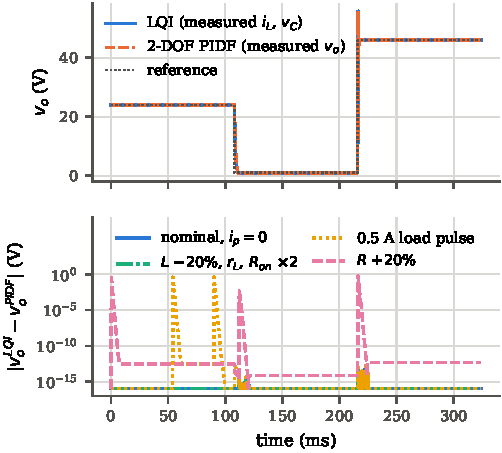
\includegraphics[width=\columnwidth]{figures/fig_equivalence.pdf}
\caption{Top: LQI with measured $(i_L,v_C)$ and its 2-DOF PIDF with measured $v_o$ on the reference mission (continuous time, averaged nonlinear plant, saturation active). Bottom: absolute output difference; the nominal and inductor-branch-mismatch curves lie at the floating-point floor, the load-pulse and load-mismatch curves show the predicted departures.}
\label{fig:equiv}
\end{figure}


\subsection{Seven algorithms on the LQI-weight space}\label{sec:res:algos}
Table~\ref{tab:algores} and Fig.~\ref{fig:campaign}(a) summarize the 180 runs of
the CMO--LQI--PIDF family. \CMOfeas{} runs end feasible. All six branches
converge to the same optimum: their best records lie between \CMObestLo{} and
\CMObestHi{}, a spread of $2\times10^{-4}$, and decode to practically the same
controller. The LQI-weight space therefore has a single, well-defined optimum
under the 33 inequalities, and the retained design is not an artefact of one
operator or one seed. The retained record improves the normalized objective by
\CMOgainPct{}\,\% with respect to the Bryson record $\xi_0$, while $\xi_0$
itself violates the overshoot specification.

What separates the operators is reliability, not the optimum. The Friedman test
over matched seeds rejects equality ($Q=\FriedQ$, $p=\FriedP$); after Holm
correction \HolmNsig{} pairwise difference remains (\HolmSig{}). pIGWO reaches a
feasible design in 28 of 30 seeds and pAEABC in 25, against 13 for GA. The
refinement stage matters most where the global stage is weakest: it lowers the
median final score by \CMOrefineABC{}\,\% for ABC and \CMOrefineAE{}\,\% for
pAEABC, and it is what turns several infeasible global records into feasible
ones. A practitioner who can afford only one run should therefore prefer the
grey-wolf or adaptive-bee variant followed by refineBO; one who can afford a
few seeds can use any of the six.

\begin{table}[t]
\centering
\caption{CMO--LQI--PIDF family: 30 matched seeds per algorithm (Algorithms 1--6, each followed by refineBO). $J_s$ statistics over feasible runs; ``global counts runs already feasible after the 240 global calls.}
\label{tab:algores}
\footnotesize
\resizebox{\columnwidth}{!}{%
\begin{tabular}{@{}lrrrrrr@{}}
\toprule
Algorithm & feasible & global & best $J_s$ & median & IQR & mean rank\\
\midrule
PSO & 18/30 & 18/30 & 0.8152 & 0.8283 & 0.0208 & 3.77\\
GA & 13/30 & 13/30 & 0.8151 & 0.8330 & 0.0190 & 4.23\\
ABC & 17/30 & 8/30 & 0.8152 & 0.8163 & 0.0162 & 3.77\\
pAEABC & 25/30 & 18/30 & 0.8151 & 0.8161 & 0.0177 & 2.77\\
pIGWO & 28/30 & 27/30 & 0.8153 & 0.8308 & 0.0205 & 3.10\\
pIGWO-DLH & 23/30 & 18/30 & 0.8152 & 0.8291 & 0.0256 & 3.37\\
\bottomrule
\end{tabular}}
\end{table}


\begin{figure*}[t]
\centering
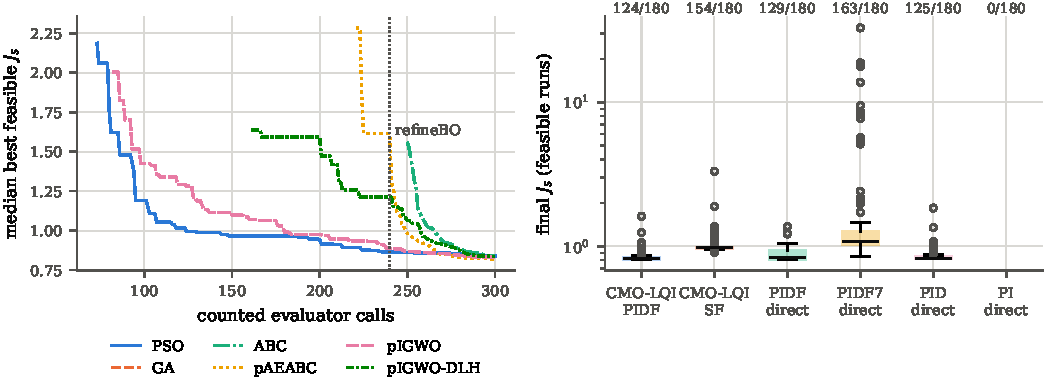
\includegraphics[width=\textwidth]{figures/fig_campaign.pdf}
\caption{(a) Median best-feasible objective against counted calls for the CMO--LQI--PIDF family (dotted line: end of the global stage). (b) Final objective of the feasible runs of every family under the identical protocol, with the number of feasible runs out of 180 above each box.}
\label{fig:campaign}
\end{figure*}

\paragraph{Retained controller}
The retained weights are $\Delta_i=\SI{\RetDi}{A}$, $\Delta_v=\SI{\RetDv}{V}$,
$\omega_B=\SI{\RetwB}{rad/s}$, giving $K=\RetK$ and closed-loop poles \RetPoles.
Its exact realization is
\begin{equation}
\theta^\star=[K_p,K_i,K_d,N,b,c,K_b]=[\RetKp,\ \RetKi,\ \RetKd,\ 2\times10^5,\ 1,\ 0,\ \RetKb].
\end{equation}
Being an LQI law, it inherits the full-state LQR margins (minimum return
difference 1, phase margin \RetPM{}), and the common-$P$ certificate over the
operating polytope gives $\alpha_{cert}=\SI{\RetAlpha}{rad/s}$ and
$\zeta_{cert}=\RetZeta$, i.e.\ \RetAlphaRatio{} times the guaranteed decay rate
of $\xi_0$ at slightly better guaranteed damping. None of these certificates is
available for a gain vector found by direct search.

\subsection{Does the LQI parameterization help? Six families, one protocol}\label{sec:res:families}
Table~\ref{tab:families} and Fig.~\ref{fig:campaign}(b) compare six families
run under the identical protocol, so that the only difference between two rows
is the space in which the seven algorithms search.

\paragraph{Same structure, different coordinates} PIDF-direct searches the
same 2-DOF PIDF ($b=1$, $c=0$, $N=N_C$) directly in
$(\log K_p,\log K_i,\log K_d,\log K_b)$ over the gain ranges spanned by the LQI
box. It reaches the same optimum (best $J_s=\BestPIDF$ against \CMObest{}) with
a similar number of feasible runs (\FeasPIDF{} against \CMOfeas{} of 180), and
the paired comparison on the same (algorithm, seed) cells is not significant
($p=\AbPIDFp$). The LQI coordinates therefore do not make the search easier
on this problem. What they change is what every candidate is. Inverting the map
\eqref{eq:map} and applying Kalman's return-difference condition shows that the
best direct-search design is itself LQ-optimal, $K=\IObestK$ with
$\min_\omega|1+L_K(j\omega)|=1$, i.e.\ the gain search converges onto the LQ
manifold; yet only \IOk{} of its \IOn{} feasible designs satisfy the condition,
so \IOpct\,\% of the controllers an equally lucky gain search may return carry
no LQ optimality, no guaranteed margins and no reason to be certifiable. The
LQI parameterization confines the search to that manifold from the first
evaluation, at no cost in optimality.

\paragraph{Richer and poorer structures} PID-direct (backward-difference
derivative) reaches best $J_s=\BestPID$ in \FeasPID{} feasible runs and is not
significantly different from CMO--LQI--PIDF ($p=\AbPIDp$). PIDF7-direct, with
free filter pole and setpoint weights, finds more feasible runs (\FeasPIDFs)
but a worse optimum (\BestPIDFs), with $N=\PIDFsN$\,rad/s, $b=\PIDFsb$ and
$c=\PIDFsc$; on the switched mission this design holds the \SI{1}{V} level
with \SwPIDFsEss{}\,mV of error and IAE \SwPIDFsIAE{}\,V\,s, i.e.\ the extra
freedom buys switched robustness at the price of the averaged objective. PI-direct never becomes feasible (minimum
violation \ViolPI{}): a PI cannot meet the overshoot, load-deviation and
current specifications of the six scenarios at once, and the paired comparison
is decisive ($p=\AbPIp$).

\paragraph{The full-state twin} CMO--LQI--SF uses the same four variables but
applies the gain as a measured-state LQI. It is feasible more often
(\FeasSF{} runs) but at a worse averaged optimum (\BestSF) than its
output-feedback realization ($p=\AbSFp$ in favour of the PIDF on the averaged
objective). On the switched mission the ordering reverses
(Section~\ref{sec:res:switched}): the twin is the more robust controller at the
\SI{1}{V} level, which is the switched counterpart of the output-current term
of \eqref{eq:gap}.

\paragraph{What the protocol, rather than the parameterization, buys}
Every family tuned under the constrained multi-fidelity protocol ends close to
full compliance on the reference mission (Table~\ref{tab:switched}: $u$ between
\SwPIdUtil{} and \SwUtil{}; the lowest value belongs to a slow PI whose IAE,
\SwPIdIAE{}\,V\,s, is 2.6 times that of the others), whereas the six fixed-rule designs lie between
\SwLQIUtil{} and \SwLQRUtil{}. The decisive ingredients are the
engineering-unit specification and the switched transition screen; the choice
of search coordinates decides the guarantees that come with the result.


\begin{table*}[t]
\centering
\caption{Controller families under the identical protocol (7 algorithms, 30 seeds, 300 calls, 33 inequalities). Paired comparison with CMO--LQI--PIDF on the same (algorithm, seed) cells: Deb-consistent score, two-sided Wilcoxon signed-rank test.}
\label{tab:families}
\footnotesize
\resizebox{\textwidth}{!}{%
\begin{tabular}{@{}llrrrrrl@{}}
\toprule
Family & variables & feasible runs & best $J_s$ & median $J_s$ (feasible) & CMO better / tie / worse & $p$ & min.\ violation\\
\midrule
CMO-LQI-PIDF & 4 (LQI weights, $K_b$) & 124/180 & 0.8151 & 0.8287 & -- & -- & 0.000\\
CMO-LQI-SF & 4 (same, full state) & 23/180 & 0.9424 & 0.9740 & -- & -- & 0.000\\
\bottomrule
\end{tabular}}
\end{table*}


\subsection{Switched validation on the reference mission}\label{sec:res:switched}
Table~\ref{tab:switched} and Fig.~\ref{fig:switched} report the frozen
controllers on the \SI{324}{ms} mission of the reference model. The energy
balance closes to better than \RESmax{} of the input energy for every row, so
all efficiency and loss figures are resolved by the integrator.

\begin{table*}[t]
\centering
\caption{Switched replay on the 324 ms reference mission (24$\to$1$\to$46 V, 0.5 A load pulse). Specification ratios: overshoot/1.5 V, load deviation/0.5 V, peak $i_L$/23 A, worst steady error/25 mV, steady duty peak-to-peak/0.20; a ratio $\le1$ meets the specification. $u$ is the largest ratio. Energy residual below \RESmax{} for every row.}
\label{tab:switched}
\footnotesize
\resizebox{\textwidth}{!}{%
\begin{tabular}{@{}lrrrrrrrrrrc@{}}
\toprule
Controller & IAE (V\,s) & overshoot (V) & $i_{L,pk}$ (A) & $|\bar e|_{\max}$ (mV) & load dev.\ (V) & $\eta$ (\%) & $E_{loss}/E_u$ & sat.\ frac. & $u$ & specs met & sensors\\
\midrule
CMO--LQI--PIDF (retained, $v_o$ only) & 0.0364 & \textbf{0.02} & \textbf{22.44} & 25.6 & \textbf{0.137} & 97.978 & 0.01801 & 0.089 & 1.02 & 4/5 & $v_o$\\
CMO--LQI--SF (twin, measured $i_L$) & 0.0348 & \textbf{0.02} & \textbf{22.70} & \textbf{0.0} & \textbf{0.214} & 97.980 & 0.01799 & 0.010 & 0.99 & 5/5 & $v_o,i_L,i_C$\\
Bryson LQI--PIDF $\xi_0$ & 0.0340 & 8.05 & 32.50 & \textbf{0.0} & \textbf{0.193} & 97.936 & 0.01845 & 0.012 & 5.37 & 3/5 & $v_o$\\
PI (loop shaping) & 0.0480 & 26.63 & 40.78 & \textbf{0.1} & \textbf{0.474} & 97.813 & 0.01972 & 0.012 & 17.76 & 3/5 & $v_o$\\
PID (pole--zero) & 0.0467 & 28.64 & 40.77 & \textbf{11.3} & \textbf{0.128} & 97.802 & 0.01984 & 0.093 & 19.09 & 3/5 & $v_o$\\
PIDF (Type III) & 0.0453 & 28.65 & 40.78 & \textbf{0.0} & \textbf{0.157} & 97.801 & 0.01986 & 0.013 & 19.10 & 3/5 & $v_o$\\
LQR & 0.1339 & \textbf{0.97} & 24.36 & 754.3 & 0.805 & 97.969 & 0.01811 & 0.001 & 30.17 & 2/5 & $v_o,i_L,i_C$\\
LQG & 0.0716 & \textbf{0.28} & 24.39 & 289.5 & \textbf{0.466} & 97.960 & 0.01818 & 0.000 & 11.58 & 3/5 & $v_o$\\
LQI (discrete, full state) & 0.0348 & 9.41 & 32.61 & \textbf{0.0} & 0.552 & 97.931 & 0.01849 & 0.013 & 6.28 & 2/5 & $v_o,i_L,i_C$\\
\bottomrule
\end{tabular}}
\end{table*}


\begin{figure*}[t]
\centering
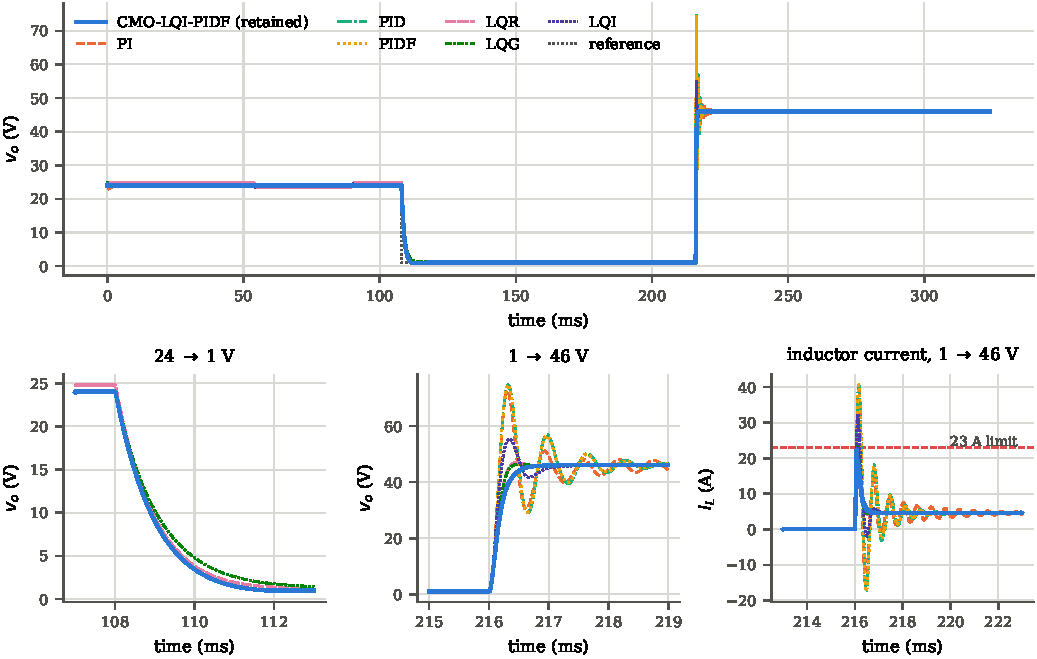
\includegraphics[width=\textwidth]{figures/fig_switched.pdf}
\caption{Switched replay on the reference mission: retained CMO--LQI--PIDF and the six fixed-rule comparators. Bottom: 24$\to$1~V and 1$\to$46~V transitions and the inductor current on the 1$\to$46~V step against the \SI{23}{A} device limit.}
\label{fig:switched}
\end{figure*}

\paragraph{Answer to the comparison question}
Against the six classical designs the result is unambiguous on the
specification, and nuanced on individual indices.
\begin{itemize}
\item \emph{PI, PID and PIDF} designed by standard frequency-domain rules hold
  every level but overshoot the 1$\to$46~V step by \SwPIOS--\SwPIDFOS{}\,V and
  draw \SwPIIpk--\SwPIDFIpk{}\,A, i.e.\ 1.8 times the \SI{23}{A} device rating;
  their specification ratios are \SwPIUtil--\SwPIDFUtil.
\item \emph{LQR and LQG}, having no integral action, leave offsets of
  \SwLQREss{} and \SwLQGEss{}\,mV at the worst level.
\item \emph{LQI}, synthesized from the same Bryson limits and reading the full
  state, tracks well (IAE \SwLQIIAE{}\,V\,s) but overshoots by \SwLQIOS{}\,V and
  peaks at \SwLQIIpk{}\,A.
\item The retained \emph{CMO--LQI--PIDF}, reading $v_o$ only, removes the
  overshoot, stays at \SwIpk{}\,A, keeps the load deviation at \SwLD{}\,V and
  reaches the highest efficiency of the output-feedback designs
  (\SwEta{}\,\%). Its IAE, \SwIAE{}\,V\,s, is within 5\,\% of the LQI and 7\,\% of
  $\xi_0$, whose lower IAE is bought with 8--\SI{9}{V} of overshoot. It misses
  one of the five mission specifications by a small margin: \SwEss{}\,mV of
  steady error at \SI{1}{V} for a \SI{25}{mV} limit ($u=\SwUtil$).
\item Its full-state twin \emph{CMO--LQI--SF}, with the same weights and a
  measured inductor current, meets all five specifications ($u=\SwSFUtil$) with
  IAE \SwSFIAE{}\,V\,s and the highest efficiency of the table (\SwSFEta{}\,\%).
\end{itemize}
The method is therefore superior to the six comparators in the sense that
matters to an industrial user: it is the only design procedure of the table that
delivers a controller within the device rating and without overshoot on the
full range, and its best controller misses full compliance by \SwEss{}\,mV
at the \SI{1}{V} level, where the converter spends a sixth of its time in
discontinuous conduction. It does not dominate every index: the LQI and
$\xi_0$ track slightly better in IAE, at the cost of 8--\SI{9}{V} of overshoot
and 32--\SI{33}{A} of peak current.

\paragraph{The value of the current sensor}
The only controller that meets every specification is the full-state twin. By
Proposition~\ref{prop:struct} the twin and the PIDF differ only by the term
$-K_{ix}(i_o-v_o/R)$ of \eqref{eq:gap}, an instantaneous feedback on the
unmodelled output current. At \SI{1}{V} in discontinuous conduction the
output-current estimate $v_o/R$ is least accurate relative to the signal, and
the PIDF must remove the resulting bias through its integrator in the presence
of a switching limit cycle; the twin removes it directly. The gap between the
two rows of Table~\ref{tab:switched} is thus the measured dividend of one
current sensor, predicted in sign and location by the theory.

\subsection{Limitations}
The evidence is simulated. The switched replica reproduces the controller-independent
figures of the reference Simulink model and its fixed comparators, but the
final numbers of Table~\ref{tab:switched} should be regenerated on the
\texttt{.slx} with the provided S-function before being quoted as Simulink
results. Losses are the modelled conduction and snubber losses of the declared
boundary; dynamic switching loss, reverse recovery, magnetic and thermal effects
are outside it, and the efficiency differences between rows (a few hundredths
of a percentage point) are far below the accuracy of a laboratory power
analyser. Component tolerances were not supplied and are not claimed: the
common-$P$ certificate covers the nominal operating polytope only. The mission
and the specification are those of a fixed \SI{48}{V} source; line regulation
is outside the study. Finally, the specification set was revised twice during
pilot campaigns that are reported in Section~\ref{sec:problem}; the final
campaign was run once, with the protocol frozen, and its switched validation
was not used for selection.
